\documentclass[degree=bachelor, tocarialchapter]{thuthesis}
% 选项
%   degree=[bachelor|master|doctor|postdoctor], % 必选,学位类型
%   secret,                % 可选(默认:关闭),是否有密级
%   tocarialchapter,       % 可选(默认:关闭),章目录中使用黑体(这项表示同时打开下面两项)
%   tocarialchapterentry,  % 可选(默认:关闭),单独控制章标题在目录中使用黑体
%   tocarialchapterpage,   % 可选(默认:关闭),单独控制章页码在目录中使用黑体
%   pifootnote,            % 可选(默认:关闭),页脚编号采用 pifont 字体符号,建议打开

% 所有其它可能用到的包都统一放到这里了,可以根据自己的实际添加或者删除。
\usepackage{thuthesis}

% 定义所有的图片文件在 figures 子目录下
\graphicspath{{figures/}}

% 可以在这里修改配置文件中的定义。导言区可以使用中文。
% \def\myname{薛瑞尼}

\begin{document}

%%% 封面部分
\frontmatter
\thusetup{
  %******************************
  % 注意:
  %   1. 配置里面不要出现空行
  %   2. 不需要的配置信息可以删除
  %******************************
  %
  %=====
  % 秘级
  %=====
  secretlevel={秘密},
  secretyear={10},
  %
  %=========
  % 中文信息
  %=========
  ctitle={威胁情报数据融合与推送服务系统},
  cdegree={工学学士},
  cdepartment={计算机科学与技术系},
  cmajor={计算机科学与技术},
  cauthor={黄锐皓},
  csupervisor={尹霞教授},
  cassosupervisor={段海新教授}, % 副指导老师
  ccosupervisor={张甲教授}, % 联合指导老师
  % 日期自动使用当前时间,若需指定按如下方式修改:
  % cdate={超新星纪元},
  %
  % 博士后专有部分
  cfirstdiscipline={计算机科学与技术},
  cseconddiscipline={系统结构},
  postdoctordate={2009年7月——2011年7月},
  id={编号}, % 可以留空: id={},
  udc={UDC}, % 可以留空
  catalognumber={分类号}, % 可以留空
  %
  %=========
  % 英文信息
  %=========
  etitle={An Introduction to \LaTeX{} Thesis Template of Tsinghua University v\version},
  % 这块比较复杂,需要分情况讨论:
  % 1. 学术型硕士
  %    edegree:必须为Master of Arts或Master of Science(注意大小写)
  %             “哲学、文学、历史学、法学、教育学、艺术学门类,公共管理学科
  %              填写Master of Arts,其它填写Master of Science”
  %    emajor:“获得一级学科授权的学科填写一级学科名称,其它填写二级学科名称”
  % 2. 专业型硕士
  %    edegree:“填写专业学位英文名称全称”
  %    emajor:“工程硕士填写工程领域,其它专业学位不填写此项”
  % 3. 学术型博士
  %    edegree:Doctor of Philosophy(注意大小写)
  %    emajor:“获得一级学科授权的学科填写一级学科名称,其它填写二级学科名称”
  % 4. 专业型博士
  %    edegree:“填写专业学位英文名称全称”
  %    emajor:不填写此项
  edegree={Doctor of Engineering},
  emajor={Computer Science and Technology},
  eauthor={Xue Ruini},
  esupervisor={Professor Zheng Weimin},
  eassosupervisor={Chen Wenguang},
  % 日期自动生成,若需指定按如下方式修改:
  % edate={December, 2005}
  %
  % 关键词用“英文逗号”分割
  ckeywords={\TeX, \LaTeX, CJK, 模板, 论文},
  ekeywords={\TeX, \LaTeX, CJK, template, thesis}
}

% 定义中英文摘要和关键字
\begin{cabstract}
  网络漏洞扫描工具是一种用于搜索网络主机中漏洞的工具,它依赖于各种已知漏洞组成的漏洞库。
  本文利用互联网设备搜索引擎,对其数据进行融合,然后和CVE信息进行比对,
  提出了一种新的检测网络主机漏洞的方法,弥补了扫描工具漏洞库更新不及时等不足,并实现了这样的一个系统,
  能够监测目标主机上可能存在的威胁,并在出现威胁时及时通知用户。我们将在文中讨论本系统的设计与实现中的细节。

  论文摘要的书写应力求精确、简明。切忌写成对论文书写内容进行提要的形式,尤其要避
  免“第 1 章……;第 2 章……;……”这种或类似的陈述方式。

  本文介绍清华大学论文模板 \thuthesis{} 的使用方法。本模板符合学校的本科、硕士、
  博士论文格式要求。

  本文的创新点主要有:
  \begin{itemize}
    \item 用例子来解释模板的使用方法;
    \item 用废话来填充无关紧要的部分;
    \item 一边学习摸索一边编写新代码。
  \end{itemize}

  关键词是为了文献标引工作、用以表示全文主要内容信息的单词或术语。关键词不超过 5
  个,每个关键词中间用分号分隔。(模板作者注:关键词分隔符不用考虑,模板会自动处
  理。英文关键词同理。)
\end{cabstract}

% 如果习惯关键字跟在摘要文字后面,可以用直接命令来设置,如下:
% \ckeywords{\TeX, \LaTeX, CJK, 模板, 论文}

\begin{eabstract}
   An abstract of a dissertation is a summary and extraction of research work
   and contributions. Included in an abstract should be description of research
   topic and research objective, brief introduction to methodology and research
   process, and summarization of conclusion and contributions of the
   research. An abstract should be characterized by independence and clarity and
   carry identical information with the dissertation. It should be such that the
   general idea and major contributions of the dissertation are conveyed without
   reading the dissertation.

   An abstract should be concise and to the point. It is a misunderstanding to
   make an abstract an outline of the dissertation and words ``the first
   chapter'', ``the second chapter'' and the like should be avoided in the
   abstract.

   Key words are terms used in a dissertation for indexing, reflecting core
   information of the dissertation. An abstract may contain a maximum of 5 key
   words, with semi-colons used in between to separate one another.
\end{eabstract}

% \ekeywords{\TeX, \LaTeX, CJK, template, thesis}

% 如果使用授权说明扫描页,将可选参数中指定为扫描得到的 PDF 文件名,例如:
% \makecover[scan-auth.pdf]
\makecover

%% 目录
\tableofcontents

%% 符号对照表
\begin{denotation}[3cm]
\item[HPC] 高性能计算 (High Performance Computing)
\item[cluster] 集群
\item[Itanium] 安腾
\item[SMP] 对称多处理
\item[API] 应用程序编程接口
\item[PI] 聚酰亚胺
\item[MPI] 聚酰亚胺模型化合物,N-苯基邻苯酰亚胺
\item[PBI] 聚苯并咪唑
\item[MPBI] 聚苯并咪唑模型化合物,N-苯基苯并咪唑
\item[PY] 聚吡咙
\item[PMDA-BDA]	均苯四酸二酐与联苯四胺合成的聚吡咙薄膜
\item[$\Delta G$] 活化自由能 (Activation Free Energy)
\item[$\chi$] 传输系数 (Transmission Coefficient)
\item[$E$] 能量
\item[$m$] 质量
\item[$c$] 光速
\item[$P$] 概率
\item[$T$] 时间
\item[$v$] 速度
\item[劝学] 君子曰:学不可以已。青,取之于蓝,而青于蓝;冰,水为之,而寒于水。木
  直中绳。輮以为轮,其曲中规。虽有槁暴,不复挺者,輮使之然也。故木受绳则直,金就
  砺则利,君子博学而日参省乎己,则知明而行无过矣。吾尝终日而思矣,不如须臾之所学
  也;吾尝跂而望矣,不如登高之博见也。登高而招,臂非加长也,而见者远;顺风而呼,
  声非加疾也,而闻者彰。假舆马者,非利足也,而致千里;假舟楫者,非能水也,而绝江
  河,君子生非异也,善假于物也。积土成山,风雨兴焉;积水成渊,蛟龙生焉;积善成德,
  而神明自得,圣心备焉。故不积跬步,无以至千里;不积小流,无以成江海。骐骥一跃,
  不能十步;驽马十驾,功在不舍。锲而舍之,朽木不折;锲而不舍,金石可镂。蚓无爪牙
  之利,筋骨之强,上食埃土,下饮黄泉,用心一也。蟹六跪而二螯,非蛇鳝之穴无可寄托
  者,用心躁也。—— 荀况
\end{denotation}



%%% 正文部分
\mainmatter
\chapter{引言}
\label{cha:intro}

\section{背景}
在互联网高度发达的21世纪,我们可以享用各种网络服务,比如浏览网页,收发邮件,文件共享等等;
互联网产业也在飞速发展,世界市值前十的公司里面有7家都是互联网公司,我们每天都在使用它们的产品,
给我们的日常生活带来了巨大的变化。但是,“机遇与风险并存”,在我们享用互联网带来的便利的同时,
互联网还带来了许多负面的问题,其中一个重中之重就是网络安全问题。

网络安全问题是在互联网中的计算机由于受到恶意的攻击,导致的软件或者硬件受到损害,
比如破坏、更改或者泄露所引起的问题。著名的网络安全问题就比如2017年5月12日开始的“永恒之蓝”\cite{ehrenfeld2017wannacry}——
全球范围内爆发的基于Windows网络共享协议进行攻击传播的蠕虫恶意代码的网络攻击事件,全世界有诸多高校内网、
大型企业内网和政府机构受到攻击,造成的损失不计其数。实际上,在该漏洞爆发之前,微软就已经发布了这个漏洞的补丁,
但是,用户并没有对自己的计算机上的漏洞有所了解以及重视,才会不幸受到黑客的攻击,如果能提前知道计算机上的漏洞就能未雨绸缪。

而为了解决这样的网络安全的问题,漏洞扫描工具应运而生。漏洞扫描工具是一种检测目标系统存在的漏洞和弱口令的工具,
可以监测目标中的通用漏洞。它们一般通过一系列逻辑判断,指出目标上的比如缓冲区溢出等漏洞。
著名的扫描工具有Metasploit\cite{o2011metasploit},SQLMap\cite{damele2012sqlmap},Nessus\cite{thacker2006probabilistic}等。漏洞扫描工具不仅能扫描外网,因为是可以自己部署的,也可以扫描内网。

但是,既然是扫描漏洞,就必然需要一个漏洞库,现有的扫描工具都存在一个问题就是漏洞库更新不够快,
而且扫描出的漏洞也不是有已知编号的漏洞,常见的检测的漏洞比如SQL注入,XSS,CSRF等。
同时,漏洞扫描通常是进行渗透测试,可能会对系统产生不可预知的影响;因此进行扫描时,只能对已获得授权的目标进行扫描,不能对“别人”的主机进行扫描。

但是,实际上现在又有一种互联网设备搜索引擎,它们是用一些网络扫描工具,比如NMap\cite{lyon2009nmap},
扫描全网主机上的一些Fingerprint信息,然后提供给用户的搜索引擎。而这种搜索引擎每一款用的方法都不一样,
产生的结果也就不一样。因此,如果我们能对不同的互联网设备搜索引擎提供的数据进行融合,而不需要实际去扫描,
然后再和已知编号的漏洞进行对比,就能最大限度地发现目标主机上的潜在漏洞。在发现了这些潜在漏洞之后再由用户去实际判断是否真的受到这种威胁,
可以大大减轻安全维护的工作,对网络安全的研究有重要意义。


\section{项目需求}
\label{sec:requirements}

该项目的需求是寻找并实现一种发现主机威胁情报的方法,可以弥补现有扫描工具的一些不足,
如只能针对特定漏洞进行扫描,漏洞库不全,更新不及时,不够自动,需要授权,对目标可能产生不良影响等;
并且该系统也提供推送功能,在发现漏洞时推送威胁情报信息;也提供可视化工具,用户可以比较容易地操作该系统完成对主机系列的安全监测。

\section{本文贡献}
\label{sec:contributions} 

本文的贡献是基本满足了上述项目需求,设计并实现了一个威胁情报数据融合与推送服务系统。
这个系统的主要功能是监测一系列主机(域名、IP地址段等)的安全情况,
发现可能的威胁时及时地告知事先设置的邮箱或者其他联系方式。

该系统的主要特点是:
\begin{itemize}
  \item 威胁情报库完整并且更新非常及时,时刻和最新最全的CVE信息保持一致;
  \item 系统并不主动地对主机进行扫描和逻辑的判断,而是采用可以找到的互联网设备搜索引擎API并对其中的信息进行分析融合;
  \item 系统会尽可能多地获得主机系列中的全部主机,而对于每一台被发现的主机,系统会穷尽其相关信息并进行信息的融合;
  \item 主动发现威胁情报并通知,不需要操作者手动部署扫描;
  \item 系统提供了一个前端网站供直观地观察可能的威胁情报;
  \item 发现可能的威胁情报,但是并不实际检验是否真的受到该漏洞的威胁。
\end{itemize}

\section{本文结构}
\label{sec:structure}

本文共分为7章。

在第一章引言中介绍本文需求提出的背景和本文的工作;
第二章相关工作主要介绍目前现有的有关漏洞扫描的工作以及和本文的工作相关的知识背景,比如现有的扫描工具具体有哪些以及它们是如何工作的,
互联网设备搜索引擎是什么等,这些背景和后续本文的工作有很大的关系,可以说后续的工作都是以这些相关工作为背景的;
第三章系统设计着重介绍系统的整体结构以及每一部分从需求到分析到最终的设计,
不注重细节以及实际生产环境中的困难,而是高屋建瓴地介绍系统的结构与设计;第四章是第三章的后续,
从代码的角度介绍系统在实现过程中采用的方法与在实际生产环境中遇到的困难是如何克服的,以及如何提高效率和正确性;
第五章是结果检验,将介绍系统实现完成之后的特点、优势、使用方法,以及举例说明系统的正确性与用处;
第六章的总结与展望将对本文的工作进行总结,得出结论并提出本文工作的不足与可以进行改进的部分;
在最后一章致谢中将感谢为本文的完成提供帮助的人们。

\chapter{相关工作}
\label{cha:related-works}

\section{漏洞扫描工具}
\label{sec:scanners}

漏洞扫描是利用已知的漏洞数据库,对本地主机或远端主机进行脆弱性检验的一种方法,
是一种发现可利用漏洞的渗透测试,经常和防火墙和入侵检测系统结合使用以提高网络的安全性。
管理员可以根据漏洞扫描的结果来发现系统中的漏洞或者错误,在黑客攻击前做好防范的工作,避免不必要的损失。
和被动防御的防火墙和入侵检测系统相反,漏洞扫描是一种主动防御方式,可以提前发现问题,做到未雨绸缪。

而漏洞扫描工具就是可以进行漏洞扫描的工具,主要分为针对网络的、针对主机的和针对数据库的漏洞扫描工具,
而本文主要关注的是针对网络的漏洞扫描工具,意即通过网络来扫描远程计算机上的漏洞的工具。

而这之中比如Metasploit就是一款著名的网络漏洞扫描工具,它提供了数百个已知漏洞的利用工具,
可以发现目标主机上是否有相应的漏洞。在发现新漏洞时,其用户可以将漏洞添加到Metasploit的目录上,
任何使用该工具的人都可以用来检测特定系统是否受到该漏洞的威胁。Metasploit使用门槛低,易推广,
为漏洞检测的自动化和及时化做出了不可小觑的贡献。

其他地,也有SQLMap或者Netsparker这样专门针对SQL注入等特定的类型的漏洞进行扫描的工具,
还有像Nessus这样的全面的系统漏洞扫描工具和分析软件。这些扫描工具都以漏洞库为基础,
通过漏洞利用工具或者一系列逻辑判断,最终找到目标主机上的漏洞的工具。

\section{互联网设备搜索引擎}
\label{chap1:search-engines}

\subsection{Censys}
\label{sec:Censys}

Censys是一款互联网搜索引擎,它使用ZMap每天扫描整个IPv4地址空间,传言只需要45分钟就能对整个地址空间进行一次扫描,
然后搜集所有的互联网中的设备的信息,返回一份关于各种资源配置和部署信息的报告,而所谓资源就分为设备、网站或者证书。

Censys的官网上是这么介绍自己的:“Censys是一款给互联网安全从业人员提供的平台,它可以帮助发现、监视、和分析互联网中的设备。
我们有规律地探测所有的公共IP地址、热门域名,选择、管理和丰富这些搜索结果,然后通过一个搜索引擎和一套API让它变得易于理解。”

\subsection{Shodan}
\label{sec:Shodan}

Shodan经常被称为最可怕的搜索引擎,或者比Google更恐怖的搜索引擎。
它也是一款互联网设备搜索引擎,它可以搜索互联网中的各种设备,不仅仅是个人电脑,
甚至包括摄像头、打印机、路由器、红绿灯、粒子回旋加速器等等,只要是连接到互联网中的设备,
都有可能被Shodan发现。如果这些设备没有做好安全防御措施,就都有可能被Shodan随意进入。比如说默认密码,
如果在Shodan上搜索“Default Password”,会发现有不计其数的打印机的仍在使用默认用户名和密码,还有很多其他设备进入根本不需要认证,
只需要用浏览器访问即可进行连接。

在Shodan的网页上,用户可以搜索一个域名、IP地址段、甚至一种设备的名称,例如Webcam,
然后找到和关键词相关的互联网设备的信息,比如运行的服务、地理位置等。通过这些信息,
就可以分析找到互联网中的脆弱部分,侵犯用户的隐私与利益,或者作为管理员防患于未然,保护用户的利益。

\subsection{ZoomEye}
\label{sec:ZoomEye}

类似于Censys和Shodan,ZoomEye也是一款互联网设备搜索引擎,
而且是一款国产的互联网设备搜索引擎,中文名是钟馗之眼。
ZoomEye通过搜索引擎开放了他们的海量数据库,用户可以通过搜索得到主机的网站组件指纹
(如操作系统、Web应用、Web服务等)和主机设备指纹。不过,为了不被黑客大规模利用,
ZoomEye还没有完全开放,目前返回结果的条数受到了一定限制。

\section{CVE}
\label{sec:CVE}

CVE的全称是Common Vulnerabilities \& Exposures,
中文名是公共漏洞和暴露。CVE类似于一个字典表,给目前已知的漏洞一个统一的名字,
形如CVE-XXXX-XXXX,中间4位是年份,最后的几位(不一定是4位)表示实际的编号。
通过这个统一的名字,安全工作人员可以在各自的漏洞库和评估工具中共享数据,易于管理。即便如此,
不代表这些不同的工具就易于整合到一起,CVE只是提供了一个目录,或者“关键字”。

CVE的官方网站是https://cve.mitre.org,上面提供了每一个CVE的相关信息、统计信息,
用户也可以自行上传CVE或者下载CVE。而CVE Details是一个经过整理过的网站,
上面记载了所有CVE的详细信息,便于用户阅读,网址是https://www.cvedetails.com。

\section{Exploit Database}
\label{sec:Exploit-Database}

Exploit Database是一个漏洞库网站,上面有海量的漏洞利用脚本,
安全人员可以利用它来提高公司设备的安全性,网址是https://www.exploit-db.com。
其Exploits版块有Remote Exploits,用于展示最新的远程漏洞利用脚本;
Web Application Exploits,用来展示最新的Web应用漏洞利用脚本,比如SQL注入等;
Local \& Privilege Escalation Exploits等。除此之外,还有Shellcode,Papers等版块。



%%% 其它部分
\backmatter

%% 本科生要这几个索引,研究生不要。选择性留下。
% 插图索引
\listoffigures
% 表格索引
\listoftables
% 公式索引
\listofequations


%% 参考文献
% 注意:至少需要引用一篇参考文献,否则下面两行可能引起编译错误。
% 如果不需要参考文献,请将下面两行删除或注释掉。
% 数字式引用
\bibliographystyle{thuthesis-numeric}
% 作者-年份式引用
% \bibliographystyle{thuthesis-author-year}
\bibliography{ref/refs}


%% 致谢
% 如果使用声明扫描页,将可选参数指定为扫描后的 PDF 文件名,例如:
% \begin{acknowledgement}[scan-statement.pdf]
\begin{acknowledgement}
  衷心感谢导师 xxx 教授和物理系 xxx 副教授对本人的精心指导。他们的言传身教将使
  我终生受益。

  在美国麻省理工学院化学系进行九个月的合作研究期间,承蒙 xxx 教授热心指导与帮助,不
  胜感激。感谢 xx 实验室主任 xx 教授,以及实验室全体老师和同学们的热情帮助和支
  持!本课题承蒙国家自然科学基金资助,特此致谢。

  感谢 \LaTeX 和 \thuthesis\cite{thuthesis},帮我节省了不少时间。
\end{acknowledgement}


%% 附录
\begin{appendix}
\chapter{外文资料的书面翻译}

\title{一个基于互联网扫描的搜索引擎}

{\heiti 摘要:} 从揭开随机数量的发生器中的漏洞,到跟踪“心脏滴血”漏洞的进化中的影响,快速互联网扫描都为网络安全研究开启了新的领域。
然而,这项技术仍然需要进行更多的重要的工作:即使是简单的问题,比如,“什么模型的嵌入式设备更喜欢用CBC模式密码?”,需要开发一款扫描器软件,
人力地给设备分类并加标签,和网络管理员协商,并对辱骂的抱怨进行回复。在这篇论文里,我们将介绍一个基于一刻不停的互联网扫描采集的数据的,
公开的搜索引擎和数据处理设备,叫做Censys。Censys设计之初就是为了帮助研究人员解决安全相关问题,它支持协议头和很多的相关字段的全文搜索,
比如443.https.ciper。它能辨认具体的有漏洞的设备和网络,然后生成广泛使用的模式和趋势的数据报告。Censys可以在亚秒级时间内返回这些结果,
大大降低了理解构成互联网的主机的难度。我们将展示这个搜索引擎的结构,并通过实验来评估其性能。我们也将探索Censys的应用场景,
并展示这些在最近的研究中提出的问题是如何变得易于回答的。

\section{引言}
从最近骤增的基于快速互联网扫描的论文数量就可以看出,这项技术为经验驱动的安全研究开启了新的篇章。
然而即便如ZMap这样的扫描工具减少了执行大规模端口扫描工作的时间,通过互联网扫描来收集有意义的数据仍然是一项专业而且费力的工作。
回答类似“有多少HTTPS服务器更喜欢前向安全秘钥交换方式?”这样简单的问题可能需要数周的实现和调试,
减少了安全研究人员可以专注于其他更重要的问题上的时间。在这个具体的例子中,研究人员需要开发一款高性能的扫描软件,
通过HTTPS连接到正在监听443端口的主机,测试并修复一些主机因为没有完全遵从TLS协议的描述来实现而产生的问题,运行实际的扫描,
然后处理数GB的产生的结果数据。

在开始这个过程之前,安全研究人员必须和他们学院的法律和网络管理团队进行协商,来获得执行这个扫描的权限,和他们上游的网络提供商进行协调,
之后还要对辱骂的抱怨进行回应。很多学院(和独立研究者)缺乏网络设备或者行政权来执行扫描。因为这些原因,互联网扫描成为了一项鲜有研究者研究的领域,
严重地限制了这个强大的方法论的应用。

为了使互联网扫描民主化,和使研究人员可以有效地回答关于安全协议在实际中的使用和部署的问题,我们开发了Censys,
一个不仅维护了一个实时的互联网中IPv4地址空间中主机和服务的快照,而且为这些数据提供了搜索引擎和API的云服务。
和现有的主要专注于发现主机的扫描工具相比,Censys基于全部的协议握手快速地产生结果,
促进了一种社区驱动的描述爆炸性增长的网络中嵌入式主机和漏洞的方法,而且不需要或者需要很少任何用户的准备。

为了使该工具接近一个实时的互联网的鸟瞰图,Censys持续地在公共地址空间上扫描一系列重要端口和协议。
它检查这些数据的有效性并用可插拔的扫描框架并进行应用层的握手,而这个框架会仔细分析每次握手并产生关于每一个主机和协议的结构化数据。
产生的结果数据是经过后处理的,带有一个可扩展的标记框架,使得研究人员可以通过编程来定义额外的属性来分辨每个主机的设备的模型和标记和安全有关的属性。
我们透明地操作Censys并把数据直接暴露给研究社区。相应地,
我们希望外部研究人员为Censys贡献扫描软件(用来扫描更多的协议)和标记(用来分辨设备或属性)。以这种方法,Censys把扫描的机械操作自动化且中心化。

Censys把结果通过一个公开的搜索引擎,REST API,所有人都可以访问的Google BigQuery中的表和可以下载的数据集返回给研究人员。
搜索的接口使得研究人员可以进行全文搜索,也可以查询任意在扫描后和后处理后的结构化的字段和标记(比如443.https.cipher\_suite)。
它支持全文搜索,正则表达式搜索,和数据范围搜索,而且查询可以含有布尔逻辑。这些查询可以和谁都可以访问的目前的IPv4主机,
Alexa Top 1 Million中的网站和已知的X.509证书的快照进行竞争。在执行一次搜索后,用户可以互动地发现他们搜索的主机,站点和证书,
同时也会生成在研究中可以直接使用的数据报告。

举个简单的例子,Censys可以简单地通过443.https.heartbleed.vulnerable: true AND location.country\_code: 
US这条搜索词来分辨在美国的主机中有“心脏滴血”漏洞的主机。从这里,Censys可以输出一个完整的匹配的IP地址的列表,
并且能绘制出最常见的漏洞设备模型的分布图。这些查询都是在1秒内完成的。

为了便于更复杂的分析,我们发布原始应用程序握手和日常的时间点快照的结构化数据。 
这些数据可以通过SQL语句查询可公开访问的Google BigQuery表获得或以JSON格式下载。Censys的另一个提供数据的方式是一个公开的REST API,
允许研究人员导出原始数据查询结果,获取统计数据,查看特定主机和网络的历史状态。

我们将在第三部分中提供Censys的收集数据的架构,在第四部分中解释Censys如何向研究人员提供数据,并在第五部分描述我们是如何部署的。
接下来我们将在第六部分中展示Censys可以应用于轻松回答一系列有关最近的安全研究相关的问题的潜力,
其中包括衡量POODLE的影响和跟踪易受攻击的工业控制系统。

互联网扫描已经展示出应用于揭露安全问题和理解安全复杂的分布式系统的巨大的潜力。通过把扫描移到云端,Censys大大减少了调查这些问题需要的努力,使研究人员能够专注于提出更重要的问题而不是回答他们的机制。此外,Censys允许安全社区提高全球协议覆盖并提供一个易于处理的解决方案,以理解数量增加的互联网中的嵌入式设备。同时,它最大限度地减少研究小组的冗余扫描,并最小化将会到来的被网络运营商监控的网络拥堵。
Censys可以通过公开网站https://censys.io免费访问。


\section{互联网好公民}

与通过主动网络探索进行的任何研究一样,我们的工作提出了重要的伦理考虑。我们仔细考虑了实验测量并披露我们的结果的影响。在考量我们的影响时,
我们考虑了各种利益相关者,从我们当地的学院到互联网服务提供商和远程系统的所有者。虽然该社区尚未获得主动测量的健全的道德标准,
我们的考量遵循广泛的道德原则,如“门洛报告”中的内容,以及按照原来ZMap中工作方式中规定的道德规范工作。

我们和网络管理员,我们的部门、学院和机构的IT领导协商,同样也和我们的上游ISP协商,以确保我们的扫描不会对网络运营产生不利影响,
并且支持中心可以将外部查询传送给我们的团队。第二,我们表示了我们活动的良好意图。全部进行扫描的主机具有WHOIS记录并有反向DNS条目描述扫描的意图。
此外,每台进行扫描的主机在80端口上运行一个简单的网站来描述研究的目标,包括我们要收集的数据,以及如何与我们联系。
第三,我们欢迎用户的排除请求并在24小时内对请求做出回应。第四,全部扫描执行符合标准的握手; 我们不发送格式错误的数据包或握手。

公开扫描数据也会引起道德问题,因为它公开有关潜在脆弱系统的信息。为了尽量减少危害,我们故意选择收集和分发至少在原则上已经公开可见的数据。
我们的扫描器不尝试登录,部署任何攻击,或尝试访问非公共资源路径。此外,我们将退出扫描请求视为一项从搜索索引中删除的请求,
以允许远程管理员决定是否包括在Censys的公共接口中。之后,许多网络运营商在了解了我们测量工作的目标后表示支持,并邀请我们继续扫描他们。
最后,我们希望通过发布我们小心获得和妥善管理的扫描数据,我们可以减少需要由其他研究人员进行的互联网扫描,从而减轻目的地网络的整体负担。

相比之下,人们已经工人攻击者已经会通过僵尸网络和防弹托管服务提供商使用互联网扫描工具来查找存在漏洞的设备。因此,配置为公开公开数据的系统有一定风险。
Censys通过给研究人员提供可靠和符合伦理的数据的来源,使得合法的研究人员更好地研究和强化这些主机,来使这片场地平等。

\section{收集数据}

Censys的数据是通过横向扫描公共IPv4地址空间获得的,它由一系列扫描器池中的扫描器完成。首先,我们使用ZMap进行主机发现扫描,
用可插拔的应用程序扫描器与会响应的主机进行程序握手,并派生结构化字段(例如证书主体或TLS密码套件)握手。我们保存并发布原始握手,
但是也继续进一步处理,验证收集的扫描数据,提取有价值的字段和用额外的元数据标注握手,比如使用用户定义的注释的设备型号和软件版本。

结构化的带标注的数据然后流式传输到中央数据库ZDb,由其汇总水平扫描的结果,调整数据并更新综合记录,用来描述个人的IPv4主机,
Alexa Top 1 Million中的网站,以及维护所有发现的辅助收集X.509证书和公钥。ZDb流更改到下游服务并产生可发布的时间点的主机和网站的快照,
以及差量更新其证书和公钥的集合。

有几个观察导致了这个架构。首先,当横向扫描测量一项服务的一个方面时(例如,一个HTTPS服务器是否支持SSLv3),研究问题通常需要多次扫描。例如,
计算支持SSLv3的HTTPS服务器的百分比时,需要一个通用的TLS扫描和一个SSLv3扫描。同样,设备型号只能通过它的HTTP页面识别,
但是这个信息对于研究任何协议都是有用的。因此,尽管数据是根据协议收集的,但是应按主机分组。其次,我们的框架需要可扩展,并且便于社区的加入。
ZMap的成功大部分归功于用户的贡献探针模块,我们相信Censys也是如此。在嵌入式设备数量的爆炸式增长互联网,这对于标注主机和服务尤其正确。反之,
Censys需要透明地操作并将数据提供给社区。第三,扫描和标注的数量都会随着时间而增长;我们的架构应该线性变化来处理这个增加负载。

\begin{figure}[H]
  \centering
  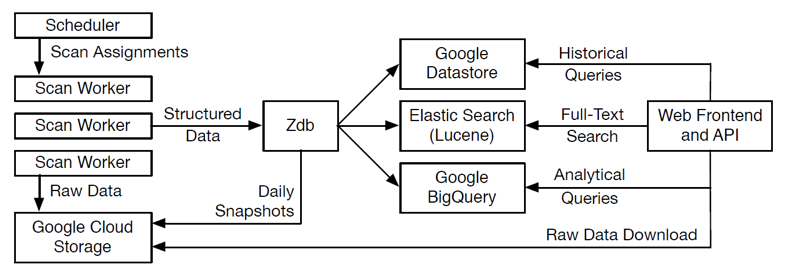
\includegraphics[scale=0.8]{censys-structure.png}
  \caption{{\heiti Censys系统体系结构} - Censys由IPv4地址空间的扫描应用程序驱动,它由一系列扫描器池中的扫描器完成。 
  这些扫描器完成扫描,提取有价值的字段,并标注记录额外的元数据,以便生成有关每个主机的结构化数据。 
  这些记录在一个中央数据库引擎ZDb中管理,它维护每个主机的当前状态。 ZDb将更新后的记录提交给Web前端,可供研究人员查询数据。}
  \label{fig:censys-structure}
\end{figure}

\subsection{互联网扫描}

在数据收集的第一步,我们使用ZMap来针对IPv4执行单包主机发现地址空间扫描。ZMap发现的主机作为可插拔应用程序扫描程序的种子,
用来执行后续的应用程序层握手并产生结构化的JSON数据,来描述主机是如何配置的的某个方面。通常情况下,
应用程序扫描程序只执行一次握手衡量服务配置的一个方面。例如,我们执行单独的横向扫描并使用不同的可插拔的扫描器来衡量HTTPS主机如何响应典型的TLS握手,
主机是否支持SSLv3,以及主机是否容易受到“心脏滴血”攻击。

{\heiti 可插拔的扫描器。}虽然我们可以使用ZMap来执行许多协议的主机发现,但是每个应用程序扫描器需要和协议相关的特定的代码,
而Censys的长期成功是因为它可以轻松添加新的协议。为了减少扫描新协议所需的工作量,Censys处理扫描的细节,并只需要最低限度的应用程序相关的扫描器。
具体而言,Censys需要一个自包含的Linux的可执行文件,它可以根据IP地址,通过stdin输入执行应用层握手,产生结构化的JSON输出,
在stdout上描述如何协议是如何配置的。Censys通过限制提供给扫描器的IP地址的速率控制网络带宽,用ZMap的内置分片工具分割扫描的多个扫描器,
并用ZMap的黑名单来保证应用程序扫描器不会扫描已经请求排除了的网络。

为了保护我们的基础设施,我们需要这个应用程序扫描程序不用root权限或内核操作修改就能工作。最后,我们鼓励研究人员输出JSON格式的扫描的元数据,
并用一个标准格式记录错误,使得Censys能够确认是否扫描已成功完成。我们希望通过要求最小的属性集,并允许语言的灵活性,
不仅可以减少我们团队添加额外的协议所需的工作量,还能鼓励外部社区开发新的扫描器。

{\heiti 扫描调度。}虽然立即测量协议的所有方面在技术上是非常简单的,但这经常涉及多次握手,这可能潜在地淹没主机(例如,
一个只允许同时一个或两个连接的嵌入式设备)。所以我们不这么做,而是选择独立执行扫描,依靠我们的数据处理流水线来聚合来自不同的数据扫描的数据,
以减少个别主机的负载。

在内部,扫描通过元组来引用(端口,协议,子协议,网络目的地),例如(443,https,heartbleed,ipv4\_shard1),
个人扫描的执行通过由扫描和时间戳引用。我们目前维护一个主扫描时间表; 我们计划自动规划扫描让它往后执行,以更好地分配网络负载。

\subsection{ZGrap:我们程序的扫描器}

我们正在发布一个快速和可扩展的应用程序扫描器,ZGrab,它符合之前描述的需求,也会促进新型扫描的快速发展。 目前,ZGrab支持HTTP,HTTP代理,
HTTPS,SMTP(S),IMAP(S),POP3(S),FTP,CWMP,SSH和Modbus的应用程序握手,以及StartTLS,Heartbleed,SSLv3和特定的密码套件检查。 
在带有Intel X520以太网适配器的双核Xeon E5-2640处理器上(6核2.5GHz),ZGrab可以在6小时20分钟内完成全部IPv4地址空间的HTTPS握手,
以及在3小时9分钟内完成一次banner-grab和所有可公开访问的SMTP的StartTLS连接主机,速度分别为1.86k和1.32k台主机每秒。

ZGrab是用Go实现的,我们选择Go是因为其原生的并发性,和其他低级语言相比安全性以及其原生的密码学库。该框架允许扫描器被定义为一个串行链的网络事件。
默认情况下,ZGrab对每台主机将只执行一个事件,连接,其行为只是打开一个TCP连接。最简单的事件可以是读取或写入数据,或更高级地,例如发起TLS握手。
例如,HTTPS扫描器被定义为一次连接事件和一次TLS握手事件。为了扩展ZGrab以支持扫描SMTP服务器之间的StartTLS支持,
我们添加了事件来读取SMTP的banner,写入SMTP EHLO命令,读取SMTP响应,发送StartTLS命令,读取响应,并执行TLS握手:总共62个LoC。
ZGrab框架处理并发连接,以及日志记录和生成描述连接的JSON文档。

原始的Censys部署中的所有协议都使用ZGrab,我们也鼓励其他研究人员考虑使用它作为开发其他应用程序扫描程序的起点。
我们正在发布和维护ZGrab作为一个独立的开源工具作为ZMap Project1的一部分。ZGrab可以独立于Censys使用,也可以结合ZMap使用:ZMap快速主机,
ZGrab产生关于每个主机的结构化数据。

\subsection{验证,提取和标注}

由可插入应用程序扫描器产生的原始JSON数据的由Censys收集,并在那里进行验证,转换成一个结构化的模式,并附加标注元数据(例如,设备制造商和型号),
然后才流入我们的中央数据库。

{\heiti 验证。}Censys以两种方式验证扫描数据。第一,我们扩展了ZMap来检测在主机发现阶段的网络响应的差异。如果扫描响应率在任何时候低于设定的阈值,
或者变化多于在扫描期间设置的数量,或者达到sendto失败的最大数量,或者如果libpcap跟不上导致丢失了设定数量的数据包,扫描自动终止并被重新安排。
其次,Censys在扫描完成时验证,并在ZMap或者应用程序扫描器的响应率低到一个静态边界时,或者在偏离之前两周的扫描的中位数超过了10\%时,拒绝这次扫描;
 被拒绝的扫描之后会手动检查。这些检查主要是为了检测瞬时网络故障,人为的配置错误和编码错误。

{\heiti 提取。}应用程序扫描仪输出与网络握手类似格式的,有关的原始数据应用程序握手的每个方面。例如,在TLS的情况下,
客户端和服务器的随机输出是客户端和服务器Hello消息的一部分。虽然这个数据是一些研究所需要的,但是很多这些字段都不是搜索主机或识别设备时有用的,
而且会导致我们的数据库中不必要的混乱。同样地,通常搜索的字段嵌套在网络的深处协议消息中,使它们很难被找到。
我们保存然后发布原始应用程序扫描器输出,但是也提取其中重要的值并转换握手数据为一种已经发布其格式的一致的结构化记录。这个过程中,
我们进一步以一种确定性的方式输出记录(即,如果没有记录更改了配置,则它们使用相同的加密哈希算法),
这使我们之后可以通过丢弃不包含更改的记录来减少负载。我们管这些表示服务配置的确定性记录叫做原子。

{\heiti 标注。}尽管应用程序扫描仪的输出可用于识别设备型号或版本,但这些细节不会被扫描器直接展示。相反,他们经常需要少量的逻辑
(例如,对HTTP服务器头或证书主体运行一个正则表达式)。为了方便添加这种类型的元数据,Censys允许研究人员定义标注 – 很小的函数 - 
可以给主机,网站和证书插入额外的元数据字段(例如,device\_module)或附加简单的标签(例如IPMI服务器的管理卡)。
注释被定义为对Censys从每次扫描生成的结构化数据只读的独立的Python函数。我们在图3中展示了一个用于标记Dell iDRAC远程管理卡的示例注释。

我们鼓励研究人员(和终端用户)贡献新类型的设备和漏洞注释。我们将在GitHub(http://github.com/zmap/ztag)
上托管我们的注释库和我们的转换和模式,作为一个独立的开源项目,ZTag。我们注意到,当ZTag与ZMap和ZGrab配合使用时,
研究人员可以独立重现Censys的数据处理流水线并产生相同的数据(图~\ref{fig:protocol})。

\begin{figure}[H]
  \centering
  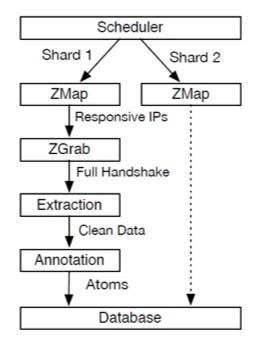
\includegraphics[scale=0.8]{protocol-scan.png}
  \caption{{\heiti 协议扫描和注释} - 每个扫描器使用ZMap执行一小部分的IPv4地址主机发现,并使用可插拔的应用程序扫描器完成协议握手。
  Censys用额外的元数据根据兴趣和注释记录提取字段。来自协议握手的信息被转换为一个原子信息 – 
  一段确定性的数据结构描述在一台主机上一个具体的协议。}
  \label{fig:protocol}
\end{figure}

\section*{翻译对应的原文索引}

\begin{translationbib}
\item Durumeric Z, Adrian D, Mirian A, et al. A search engine backed by internet-wide scanning
[C]//Proceedings of the 22nd ACM SIGSAC Conference on Computer and Communications
Security. [S.l.]: ACM, 2015: 542-553.
\end{translationbib}
\end{appendix}

%% 个人简历
\begin{resume}

  \resumeitem{个人简历}

  xxxx 年 xx 月 xx 日出生于 xx 省 xx 县。

  xxxx 年 9 月考入 xx 大学 xx 系 xx 专业,xxxx 年 7 月本科毕业并获得 xx 学士学位。

  xxxx 年 9 月免试进入 xx 大学 xx 系攻读 xx 学位至今。

  \researchitem{发表的学术论文} % 发表的和录用的合在一起

  % 1. 已经刊载的学术论文(本人是第一作者,或者导师为第一作者本人是第二作者)
  \begin{publications}
    \item Yang Y, Ren T L, Zhang L T, et al. Miniature microphone with silicon-
      based ferroelectric thin films. Integrated Ferroelectrics, 2003,
      52:229-235. (SCI 收录, 检索号:758FZ.)
    \item 杨轶, 张宁欣, 任天令, 等. 硅基铁电微声学器件中薄膜残余应力的研究. 中国机
      械工程, 2005, 16(14):1289-1291. (EI 收录, 检索号:0534931 2907.)
    \item 杨轶, 张宁欣, 任天令, 等. 集成铁电器件中的关键工艺研究. 仪器仪表学报,
      2003, 24(S4):192-193. (EI 源刊.)
  \end{publications}

  % 2. 尚未刊载,但已经接到正式录用函的学术论文(本人为第一作者,或者
  %    导师为第一作者本人是第二作者)。
  \begin{publications}[before=\publicationskip,after=\publicationskip]
    \item Yang Y, Ren T L, Zhu Y P, et al. PMUTs for handwriting recognition. In
      press. (已被 Integrated Ferroelectrics 录用. SCI 源刊.)
  \end{publications}

  % 3. 其他学术论文。可列出除上述两种情况以外的其他学术论文,但必须是
  %    已经刊载或者收到正式录用函的论文。
  \begin{publications}
    \item Wu X M, Yang Y, Cai J, et al. Measurements of ferroelectric MEMS
      microphones. Integrated Ferroelectrics, 2005, 69:417-429. (SCI 收录, 检索号
      :896KM)
    \item 贾泽, 杨轶, 陈兢, 等. 用于压电和电容微麦克风的体硅腐蚀相关研究. 压电与声
      光, 2006, 28(1):117-119. (EI 收录, 检索号:06129773469)
    \item 伍晓明, 杨轶, 张宁欣, 等. 基于MEMS技术的集成铁电硅微麦克风. 中国集成电路,
      2003, 53:59-61.
  \end{publications}

  \researchitem{研究成果} % 有就写,没有就删除
  \begin{achievements}
    \item 任天令, 杨轶, 朱一平, 等. 硅基铁电微声学传感器畴极化区域控制和电极连接的
      方法: 中国, CN1602118A. (中国专利公开号)
    \item Ren T L, Yang Y, Zhu Y P, et al. Piezoelectric micro acoustic sensor
      based on ferroelectric materials: USA, No.11/215, 102. (美国发明专利申请号)
  \end{achievements}

\end{resume}


%% 本科生进行格式审查是需要下面这个表格,答辩可能不需要。选择性留下。
% 综合论文训练记录表
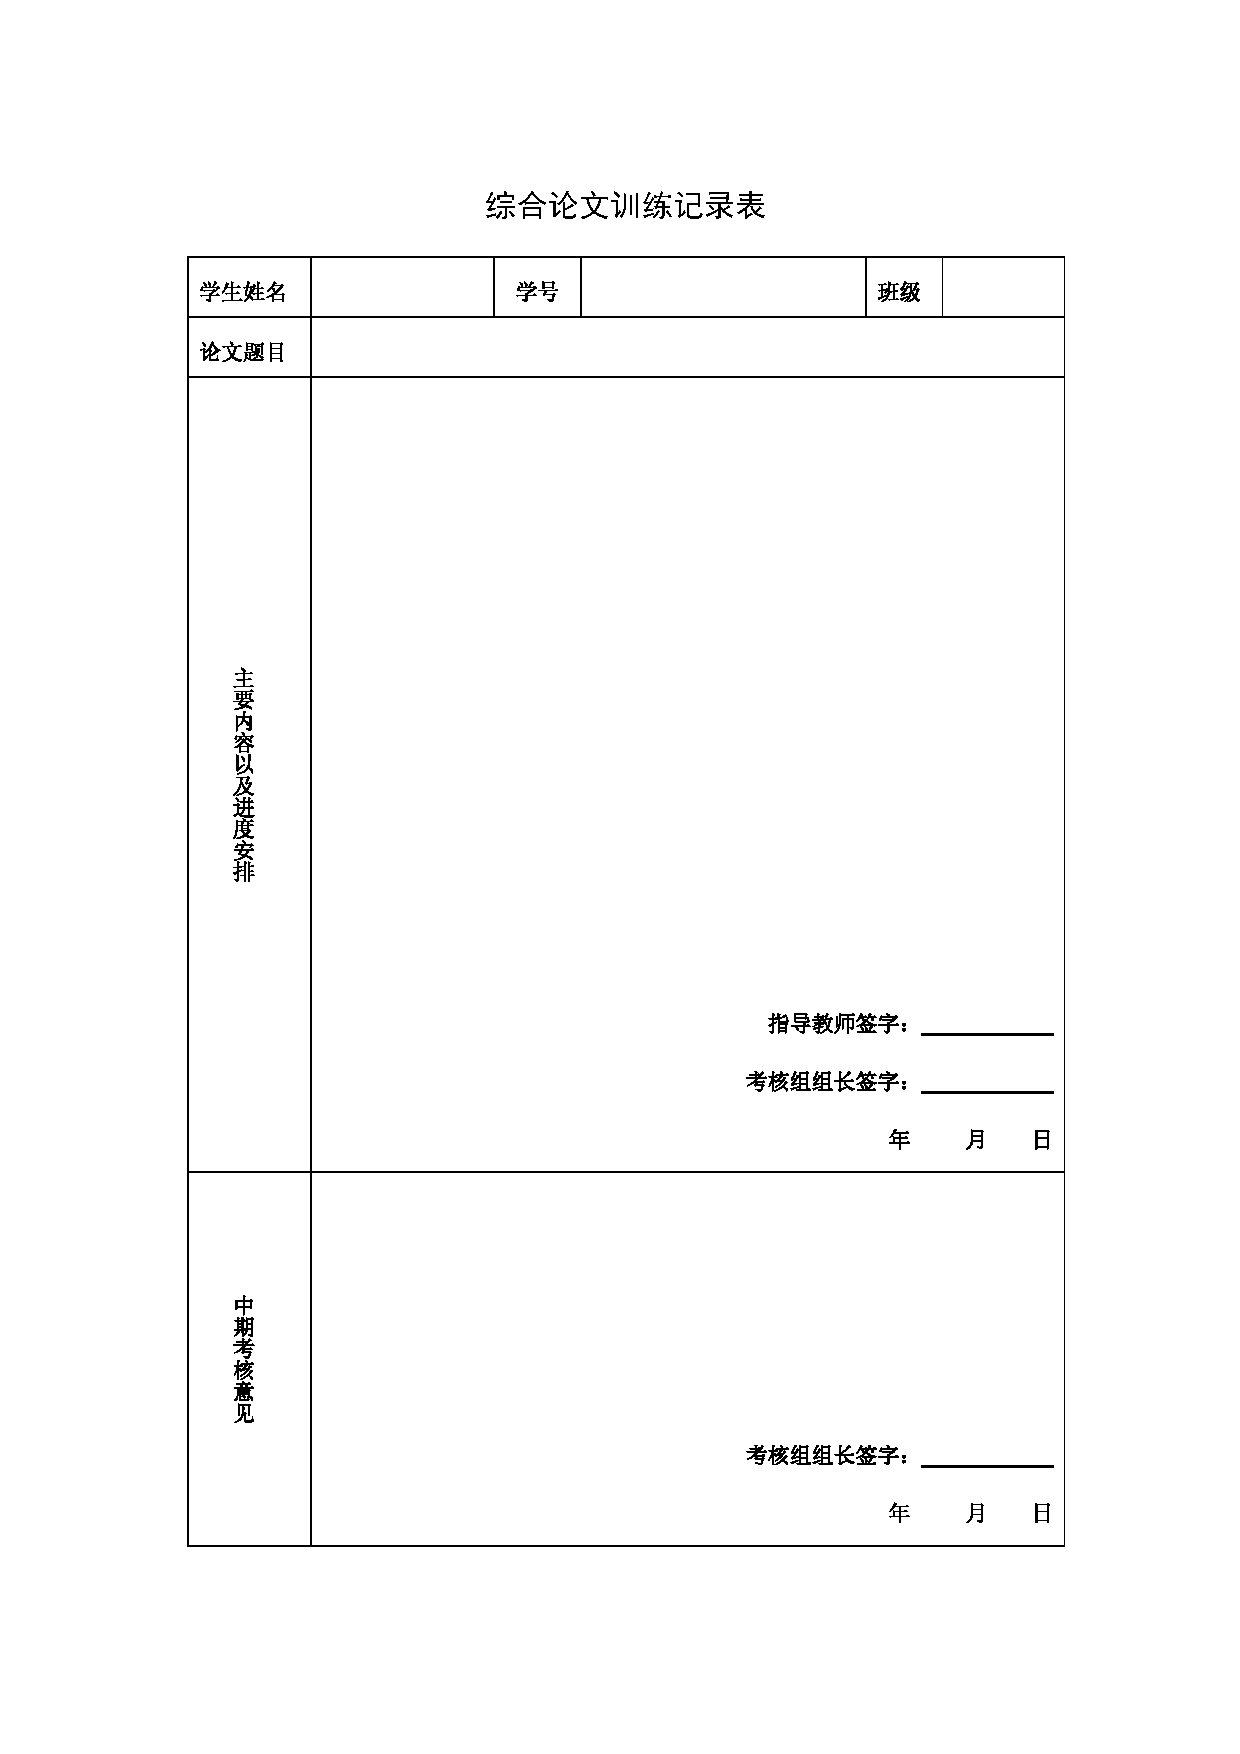
\includepdf[pages=-]{scan-record.pdf}
\end{document}
